\documentclass[../main.tex]{subfiles}

\begin{document}

Cartesian plane is $\mathbb{R}\times \mathbb{R} = \{(x,y) \mid x \in \mathbb{R} \text{ and } b \in \mathbb{R} \}$.

\begin{figure}[H]
  \centering
  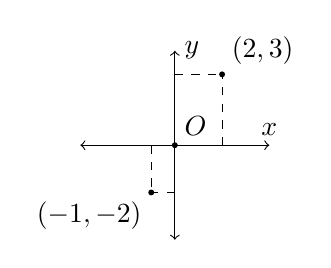
\begin{tikzpicture}[scale=0.3]
  \draw[<->] (-4,0) -- (4,0);
  \node[above] at (4,0) {$x$};
  \draw[<->] (0,-4) -- (0,4);
  \node[right] at (0,4) {$y$};
  \draw[fill] (0,0) circle [radius=0.1];
  \node[above right] at (0,0) {$O$};
  \draw[dashed] (2,0) -- (2,3);
  \draw[dashed] (0,3) -- (2,3);
  \node[above right] at (2,3) {$(2,3)$};
  \draw[fill] (2,3) circle [radius=0.1];
  \draw[dashed] (-1,0) -- (-1,-2);
  \draw[dashed] (0,-2) -- (-1,-2);
  \node[below left] at (-1,-2) {$(-1,-2)$};
  \draw[fill] (-1,-2) circle [radius=0.1];
\end{tikzpicture}
\end{figure}

Horizontal axis is usually called the $x$ axis, the vertical axis is called the $y$ axis. Intersection of the axes is called the origin, denoted $O$.

The coordinate axes divide the Cartesian plane into four quadrants.
\begin{figure}[H]
  \centering
  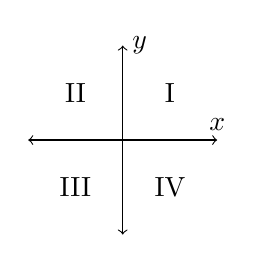
\begin{tikzpicture}[scale=0.3]
  \draw[<->] (-4,0) -- (4,0);
  \node[above] at (4,0) {$x$};
  \draw[<->] (0,-4) -- (0,4);
  \node[right] at (0,4) {$y$};
  \node at (2,2) {I};
  \node at (-2,2) {II};
  \node at (-2,-2) {III};
  \node at (2,-2) {IV};
\end{tikzpicture}
\end{figure}

By the Pythogerean Theorem, the distance of two points $(x_1, y_1)$ and $(x_2, y_2)$ is
\begin{figure}[H]
  \centering
  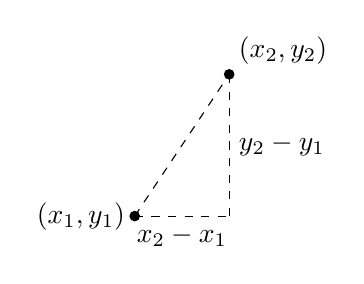
\begin{tikzpicture}[scale=0.6]
  \node[above right] at (3,4) {$(x_2,y_2)$};
  \draw[fill] (3,4) circle [radius=0.1];
  \node[left] at (1,1) {$(x_1,y_1)$};
  \draw[fill] (1,1) circle [radius=0.1];
  \draw[dashed] (1,1) -- (3,1);
  \draw[dashed] (3,1) -- (3,4);
  \draw[dashed] (1,1) -- (3,4);
  \node[below] at (2,1) {$x_2-x_1$};
  \node[right] at (3,2.5) {$y_2-y_1$};
\end{tikzpicture}
\end{figure}

The distance of $(x,y)$ to the origin $(0,0)$ is $\sqrt{x^2+y^2}$.
\begin{example}
  Find the distance between $(-1, 1)$ and $(3, -4)$.
\end{example}

\subsection*{Graphs of Equations}
The set of all points $(x,y)$ satisfying an equation in $x$ and $y$ is called the \textbf{graph of that equation}.

\begin{example}
  The graph of $x^2+y^2=4$ is the set of all $(x,y)$ whose distance to $(0,0)$ is 2, i.e. a circle with center at origin and radius 2.
\end{example}

\subsection*{Equations of Lines}
For any two points $(x_1, y_1)$ and $(x_2, y_2)$ on a non-vertical line $L$, the quantity $m=\dfrac{y_2-y_1}{x_2-x_1}$ is constant and is called the \textbf{slope} of the line $L$.

Let $L$ be a nonvertical line. Let $m$ be the slope of $L$ and $(x_1, y_1)$ be the coordinates of a point on $L$. If $(x,y)$ is another point on $L$, then
\[
  \frac{y-y_1}{x-x_1} = m
\]
Hence any $(x,y)$ on $L$ satisfies
\[
  y = m(x-x_1) + y_1
\]
The above is known as an equation for the line $L$.

All points on a \textbf{vertical line} have their $x$ coordinate equal to a constant $a$. So the equation of a vertical line is $x=a$. \textbf{Horizontal lines} have equations of the form $y=a$.

\textbf{y-intercept} of a nonvertical line $L$ is the $y$-coordinate of the point where $L$ intersects the y-axis. \textbf{x-intercept} of a nonhorizontal is defined similarly.

\begin{example}
Find an equation of the line through the points $(1,-1)$ and $(3,5)$. Draw the line. Find the x and y intercepts.
\end{example}

\begin{example}
Find an equation of the line that passes through the point $(-3,-4) $ and has slope $2$. Draw the line.
\end{example}

\begin{example}
Find the slope and the two intercepts of the line with equation $8x+5y=20$. Draw the line.
\end{example}

\subsection*{Parallel vs. perpendicular lines}
We call two lines \textbf{parallel} if their slopes are equal. We call two lines \textbf{perpendicular} if they intersect at right angles ($90^{\circ}$).

\begin{theorem}
  Two nonvertical lines with slopes $m_1$ and $m_2$ are perpendicular if and only if $m_1 m_2 = -1$.
\end{theorem}

\begin{proof}
  \begin{figure}[H]
    \centering
    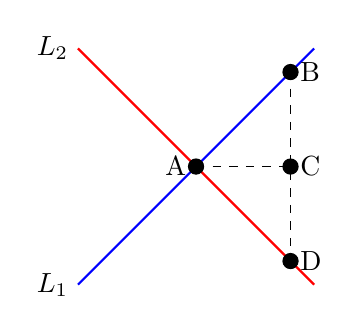
\begin{tikzpicture}[scale=1.2]
  \draw[thick, blue] (-1.25,-1.25) -- (1.25,1.25);
  \draw[thick, red] (1.25,-1.25) -- (-1.25,1.25);
  \draw[dashed] (1,1) -- (1,-1);
  \draw[dashed] (0,0) -- (1,0);
  \node[left] at (0,0) {A};
  \draw[fill] (0, 0) circle [radius=0.08];
  \node[right] at (1,1) {B};
  \draw[fill] (1, 1) circle [radius=0.08];
  \node[right] at (1,0) {C};
  \draw[fill] (1, 0) circle [radius=0.08];
  \node[right] at (1,-1) {D};
  \draw[fill] (1, -1) circle [radius=0.08];
  \node[left] at (-1.25,-1.25) {$L_1$};
  \node[left] at (-1.25,1.25) {$L_2$};
\end{tikzpicture}
  \end{figure}
  Use the similarity of the triangles ABC and DAC to get
  \[
    \frac{\abs{BC}}{\abs{AC}} = \frac{\abs{AC}}{\abs{CD}} \implies
    \frac{\abs{BC}\abs{CD}}{\abs{AC}^2} = 1
  \]
  Slope of $L_1$ ($m_1$) is $\abs{BC}/\abs{AC}=1$ and slope of $L_2$ ($m_2$) is $-\abs{CD}/\abs{AC}$. So $m_1 m_2 = -1$.
\end{proof}


\begin{example}
Find an equation of the line through $(1, -2) $ that is parallel to the line $L$ with equation $3x-2y=1$.
Draw the lines.
\end{example}

\begin{example}
Find an equation of the line through $(2,-3)$ that is perpendicular to the line $L$ with equation $4x+y=3$.
Draw the lines.
\end{example}

\end{document}
